\chapter{Zadatak G} \label{ch:g}

U ovom poglavlju je opisan i odrađen zadatak G.

\section{Opis zadatka} \label{sec:g:opis}
na temelju podataka iz f) dijela zadatka, potrebno je odrediti mehaničku energiju koju vozilo mora
utrošiti kako bi prevalilo zadanu rutu sa zadanim profilom vožnje, mehaničku energiju koju vozilo
može iskoristiti na zadanoj rutu sa zadanim profilom vožnje za regeneraciju energije. Potrebno je
prikazati krivulje svake komponente mehaničke energije zasebno i sve na jednom grafu uz ukupnu
mehaničku energiju s točno naznačenim oznakama. Dodatno, za svaku komponentu energije je
potrebno odrediti minimalnu, maksimalnu i srednju vrijednost krivulje, te prikazati je u tabličnom
obliku

\section{Rješenje} \label{sec:g:rjesenje}

Za riješenje potrebno je apsolutnei regenerativne snage iz zadatka e pomnožiti sa vremenom.
Zatim je potrebno obaviti \textit{scan\_sum} operaciju nad svim energijama kako bi se dobila
ukupna energija.

\begin{figure}
    \centering
    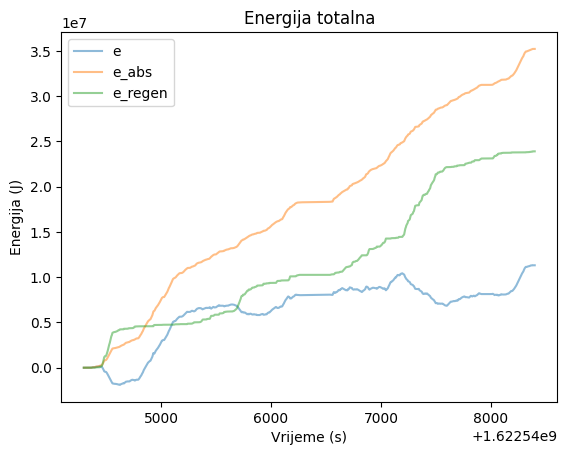
\includegraphics[width=0.8\textwidth]{images/energies_2.png}
    \caption{Prikaz izračunate energije kroz vrijeme.}
    \label{fig:g:energy_graph}
\end{figure}


\begin{table}[!ht]
    \centering
    \caption{Analiza apsolutne i renegerativne energija na vozilu}
    \begin{tabular}{llll}
    \hline
        \textbf{describe} & \textbf{e} & \textbf{e\_abs} & \textbf{e\_regen} \\ \hline
        """count""" & 9776.0 & 9776.0 & 9776.0 \\ 
        """null\_count""" & 0.0 & 0.0 & 0.0 \\ 
        """mean""" & 6.3186e6 & 1.8002e7 & 1.1684e7 \\ 
        """std""" & 3.3057e6 & 9.6363e6 & 7.1102e6 \\ 
        """min""" & -1.9022e6 & 0.0 & 0.0 \\ 
        """25\%""" & 5.9182e6 & 1.2422e7 & 5.7249e6 \\ 
        """50\%""" & 7.5995e6 & 1.8289e7 & 1.0260e7 \\ 
        """75\%""" & 8.1365e6 & 2.6147e7 & 1.6971e7 \\ 
        """max""" & 1.1334e7 & 3.5225e7 & 2.3908e7 \\ \hline
    \end{tabular}
    \label{table:c:energies2}
\end{table}
